\chapter{Methodology}\label{chap:method}

\section{Proposed Solution}

Building on the work of Gordillo et al. \cite{sgame2020}, our solution addresses key limitations in their approach. While SGAME provides a platform for creating educational video games by integrating SCORM-compliant learning objects, it has notable restrictions. Specifically, the game creation process in SGAME is confined to combining pre-existing games with a predefined set of educational questions in various fields. Furthermore, the system’s support for educational content is limited to the Spanish language, which significantly restricts its usability for users from diverse linguistic and cultural backgrounds.

To overcome these limitations, our tool is designed to provide users with greater control over the educational content they can add to their games. Unlike SGAME, which ties games to fixed educational fields, our solution allows the same game template to be adapted for different educational contexts. This approach ensures flexibility, enabling instructors to create games tailored to their specific educational needs and in their preferred language. However, we recognize that certain game templates may naturally align better with specific fields, and such constraints will be accounted for to maintain educational and gameplay coherence.

By addressing these limitations, our tool not only enhances inclusivity and usability but also fosters a more customizable and versatile approach to creating educational games, empowering instructors to provide engaging and context-specific learning experiences.

\section{System Architecture}
Since we are trying to a achive a tool that could be accessed from various devices and platforms, 
we are going to use a web-based architecture. The instructor will be using a portal to create the game, 
and share it via a link, a qr code, or a game code with the students. The students will be able to access the game from their devices, 
and the game will be able to run on any device that has a web browser. 
We also use a Baas (Backend as a Service) in the cloud to store the data of the games created, as it is shown in the figure \ref{fig:architecture}, in our case we are using Firebase.
This allows the data to be stored in the cloud, and the game to be accessed from anywhere.
The portal is creatd using Next.js, a React framework, which allows us to create a server-side rendered application.
we have developed two game templates, a space invaders-like game which was developed using unity and hosted on itch.io,
and a click-based puzzle game developed using next.js, more on those games in the next section.
\begin{figure}
    \centering
    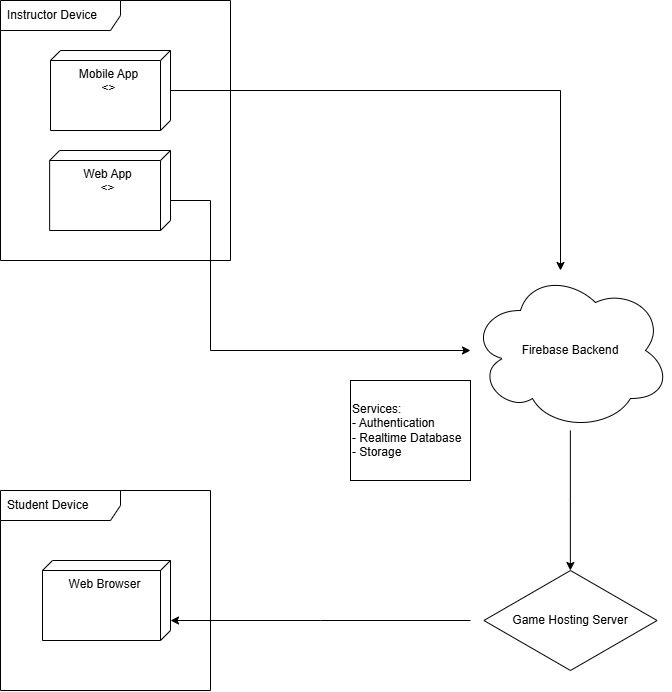
\includegraphics[width=0.8\textwidth]{figures/Deployment_UML.jpg}
    \caption{System Architecture}
    \label{fig:architecture}
\end{figure}

\section{Game Templates}
\subsection{Space Invaders-like Game}

\subsection{Click-based Puzzle Game}